\documentclass[a4paper,11pt]{article}
% ---- graphiques
\usepackage[pdftex]{graphicx}
\usepackage{wrapfig}
\usepackage{color}
\usepackage{pst-tree}
%\usepackage{hyperref}

% for accents
\usepackage[latin1]{inputenc}
\usepackage[T1]{fontenc}

\usepackage{algorithm}
\usepackage{algorithmic}

\definecolor{darkgreen}{rgb}{0,0.4,0}
\definecolor{darkblue}{rgb}{0,0,0.4}
\definecolor{darkgray}{rgb}{0.2,0.2,0.2}

% ---- inclusion de codes
\usepackage{listings}
\lstset{showstringspaces=false,tabsize=4,basicstyle=\scriptsize\sffamily,breaklines=true,breakatwhitespace=true,framexleftmargin=5mm, frame=shadowbox, framesep=1pt,rulesepcolor=\color{darkgray},rulesep=.5pt,keywordstyle=\bf\color{blue},commentstyle=\color{magenta},stringstyle=\color{red},numbers=left,numberstyle=\tiny,numbersep=5pt,columns=flexible}

\lstdefinestyle{bash}{language=bash}
\lstdefinestyle{Perl}{language=Perl}
\lstdefinestyle{Python}{language=Python}
\lstdefinestyle{C++}{language=C++,emph={__global__,__shared__,__syncthreads,blockIdx,threadIdx,float3,float4},emphstyle=\bf\color{darkgreen}}
\lstdefinestyle{DTD}{language=XML}
\lstdefinestyle{XML}{language=XML,usekeywordsintag=false,markfirstintag=true}
%begin{latexonly}
\newcommand{\includecode}[2]{
\lstinputlisting[style=#1]{#2}
}
%end{latexonly}


%\lstnewenvironment{code}{}{}
\lstnewenvironment{code_bash}{\lstset{style=bash}}{}
\lstnewenvironment{code_perl}{\lstset{style=Perl}}{}
\lstnewenvironment{code_python}{\lstset{style=Python}}{}
\lstnewenvironment{code_cpp}{\lstset{style=C++}}{}
\lstnewenvironment{code_dtd}{\lstset{style=DTD}}{}
\lstnewenvironment{code_xml}{\lstset{style=XML}}{}

\newcommand{\textcode}[1]{{\sf #1}}




\newcommand{\sofa}{SOFA}
\newcommand{\todo}[1]{}
\newcommand{\eg}{\textit{e.g.} }

\renewcommand{\vec}[1]{\ensuremath{\mathbf{#1 }}} % vector
\newcommand{\Vx}{\vec{x} } % position vector
\newcommand{\Vv}{\vec{v} } % velocity vector
\newcommand{\Va}{\vec{a} } % acceleration vector
\newcommand{\Vf}{\vec{f}} % force
\newcommand{\Vdv}{\vec{\delta\Vv}} % change of velocity vector (unknown in implicit CG, and used in constraint solver
\renewcommand{\P}{\mat{P} } % projection to a constrained space.

\newcommand{\JNL}{\mathbf{\mathcal{J}} }     % mapping des positions
\newcommand{\J}{\mat J }                 % mapping lineaire
\newcommand{\M}{\mat M }             % matrice de masse
\newcommand{\K}{\mat K }             % matrice de raideur
\newcommand{\B}{\mat B }             % matrice d'amortissement
\newcommand{\G}{\mat G }             % jacobien des contraintes



% ---- inclusion de codes
\definecolor{darkgreen}{rgb}{0,0.4,0}
\definecolor{darkblue}{rgb}{0,0,0.4}
\definecolor{darkgray}{rgb}{0.2,0.2,0.2}


% macros mathematiques
\newcommand{\ma}[1]{\ensuremath{\mathbf {#1}}}
\newcommand{\ve}[1]{\ensuremath{\mathbf {#1}}}

\usepackage{amsmath}
\usepackage{amsfonts}
\usepackage{amssymb}

% character styles
\newcommand{\bm}[1]{\ensuremath{\mathbf{{#1}}}}
\newcommand{\mcal}[1]{\mbox{$\mathcal #1$}} % rondes math
\newcommand{\bmcal}[1]{\mbox{\boldmath $\mathcal #1$}} % rondes grasses math
\newcommand{\ensemble}[1]{\mbox{$\mathbb{#1}$}}
\newcommand{\RRR}{\mbox{$\ensemble{R}^3$}} 


% d�finitions
\newcommand{\definition}[2]{\index{#1}{\bf #1}: #2}
\newcommand{\voc}[1]{\index{#1}#1}
\newcommand{\bvoc}[1]{\index{#1}{\bf #1}}

% misc
\newcommand{\EV}[1]{\stackrel{\rightarrow}{#1}}  % espace vectoriel
\newcommand{\EA}[1]{#1}                          % espace affine

% vectors, matrices
%\newcommand{\point}[1]{\mbox{$#1$}}          % un point
\newcommand{\point}[1]{\ensuremath{#1}}          % un point
\newcommand{\mat}[1]{\bm{#1}}         % matrice
\newcommand{\matnm}[3]{\bm{#1_{#2\times #3}}}  % matrice n lignes , m colonnes
\newcommand{\vect}[1]{\bm{#1}}        % vecteur 
%\newcommand{\vecf}[1]{\stackrel{\rightarrow}{#1}}  % vecteur avec fleche
\newcommand{\vecf}[1]{\mbox{$\overrightarrow{#1}$}}  % vecteur avec fleche
\newcommand{\ident}[1]{\bm{I_{#1}}}   % identit� en dimension n
\newcommand{\inv}[1]{#1^{-1}}         % matrice inverse
\newcommand{\psinv}[1]{#1^{+}}        % matrice pseudo-inverse
\newcommand{\transp}[1]{#1^T}         % transpos�e de 1
\newcommand{\trace}[1]{tr(#1)}        % trace
\newcommand{\deter}[1]{\mbox{$|#1|$}}       % determinant
\newcommand{\oppvec}[1]{\mbox{$\left( \vect {#1} \wedge \right)$}}  % operateur matriciel de produit vectoriel

% bases, reperes
\newcommand{\vecin}[2]{\mbox{${}^{#2}#1$}}    % vecteur 1 dans repere 2
\newcommand{\Base}[1]{\ensuremath{\mathcal B_{#1}}} % Symbole du repere 1
\newcommand{\chbase}[3]{\mbox{${}_{#2}^{#3}\mat{#1}$}}  % operateur 1 fait le passage de la base 3 vers la base 2
%\newcommand{\pchbase}[2]{\chbase{\mat{B}}{#1}{#2}}  % matrice de passage de la base 2 vers la base 1
\newcommand{\pchbase}[2]{\chbase{B}{#1}{#2}}  % matrice de passage de la base 2 vers la base 1
\newcommand{\Rep}[1]{\ensuremath{\mathcal R_{#1}}} % Symbole du repere 1
\newcommand{\rep}[1]{\Rep{#1}}                 % Symbole du repere 1
%\newcommand{\pchrep}[2]{\chbase{\mat{F}}{#1}{#2}}  % matrice de passage du repere 1 vers le repere 2, F comme Frame
\newcommand{\pchrep}[2]{\chbase{\bm{C}}{#1}{#2}}  % matrice de passage du repere 2 vers le repere 1

%% Operateur de passage du repere 1 par rapport a 2
%\newcommand{\ChgRep}[2]{\mbox{\boldmath $R_{#1}^{#2}$}}

% rotations	
%\newcommand{\rot}[2]{\mbox{$\mat{R}_{#1,#2}$}}      % rotation vectorielle
\newcommand{\rot}[2]{\ensuremath{\mat{R}_{#1,#2}}}      % rotation vectorielle
\newcommand{\rota}[3]{\mbox{$\mat{R}_{#1,#2,#3}$}}  % rotation affine

% translation
\newcommand{\trans}[2]{\mbox{$\chbase{\vect{t}}{#1}{#2}$}} % passage de #1 vers #2 par une translation, ou translation du repere #2 par rapport au repere #1

% vitesses et acc�l�rations
\newcommand{\VRep}[2]{\mbox{\boldmath $\dot R_{#1}^{#2}$}} % vitesse du repere 1 par rapport a 2 
%\newcommand{\Point}[2]{\mbox{\boldmath ${#1}^{#2}$}}  % Coordonnees d'un point 1 dans un repere 2
\newcommand{\Point}[2]{\mbox{$\vecin{\bm{#1}}{#2}$}}  % Coordonnees d'un point 1 dans un repere 2
\newcommand{\VPoint}[2]{\mbox{\boldmath ${\dot #1}_{/#2}$}} % Vitesse d'un point par rapport � un repere
\newcommand{\APoint}[2]{\mbox{\boldmath ${\ddot #1}_{/#2}$}} % Acceleration d'un point par rapport � un repere

% cinematique du solide
\newcommand{\derivedans}[2]{\mbox{$\dot{#1}^{(#2)}$}}  % derivee du vecteur 1 dans repere 2
\newcommand{\fixedans}[2]{\mbox{$#1_{\in #2}$}}        % vecteur 1 fixe dans repere 2
\newcommand{\vecom}{\mbox{$\bm{\Omega}$}}  % omega de 1 par rapport a 2
\newcommand{\vecrot}[2]{\mbox{$\vecom_{#1/#2}$}}  % omega de 1 par rapport a 2
\newcommand{\accrot}[2]{\mbox{$\dot{\vecom}_{#1/#2}$}}  % omega de 1 par rapport a 2
\newcommand{\vfdans}[3]{\mbox{$\vec V^{#2/#3}_{#1}$}}    % vitesse de 1 fixe dans 2 par rapport a 3
\newcommand{\afdans}[3]{\mbox{$\vec \Gamma^{#2/#3}_{#1}$}}    % acceleration de 1 fixe dans 2 par rapport a 3
\newcommand{\vmdans}[2]{\mbox{$\vec V^{/{#2}}_{#1}$}}    % vitesse de 1 mobile dans 2
\newcommand{\amdans}[2]{\mbox{$\vec \Gamma^{/#2}_{#1}$}}    % acceleration de 1 mobile dans 2

% chaines articulees
\newcommand{\liaison}[2]{\mbox{$\mathcal L_{#1,#2}$}}  % liaison du pere 1 vers fils 2 (et repere intermediaire)
\newcommand{\liaisonprime}[2]{\mbox{$\mathcal L'_{#1,#2}$}}  % deuxieme repere intermediaire de la liaison du pere 1 vers fils 2
\newcommand{\liaisonP}[2]{\mbox{$\mathcal L_{#1,#2}$}}  % Repere dans pere 1 de la liaison vers fils 2 
\newcommand{\liaisonC}[2]{\mbox{$\mathcal L'_{#1,#2}$}}  % Repere dans fils de la liaison du pere 1 vers fils 2 
%\newcommand{\transP}[2]{\pchrep{\liaisonP{#1}{#2}}{#1}}  % Matrice du repere dans pere de la liaison du pere 1 vers fils 2 
%\newcommand{\transC}[2]{\pchrep{\liaisonC{#1}{#2}}{#2}}  % Matrice du repere dans pere de la liaison du pere 1 vers fils 2 
%\newcommand{\transPC}[2]{\pchrep{\liaisonC{#1}{#2}}{\liaisonP{#1}{#2}}}  % matrice de passage entre repere liaison dans fils et repere de liaison dans pere
\newcommand{\transP}[2]{\chbase{C_p}{#2}{#1}}  % Matrice du repere dans pere de la liaison du pere 1 vers fils 2 
\newcommand{\transC}[2]{\chbase{C_c}{#2}{#1}}  % Matrice du repere dans pere de la liaison du pere 1 vers fils 2 
\newcommand{\transPC}[2]{\chbase{C_l}{#2}{#1}}  % matrice de passage entre repere liaison dans fils et repere de liaison dans pere
% \pchrep{fils}{pere} = \liaisonP{pere}{fils}\deplPC{pere}{fils}\liaisonC{pere}{fils}


\newcommand{\pctab  }{\hspace{0.15in}      }  % Pseudo-code indentation.
\newcommand{\code}[1]{ 
\begin{makeimage}
\begin{tabbing} \pctab \= \pctab \= \pctab \= \pctab \= \pctab \= \pctab \= \pctab \kill
#1
\end{tabbing}
\end{makeimage}
}
 % This file is in parent directory. Your TEXINPUTS environment variable must include .. to reach this file. Example: setenv TEXINPUTS ..:../..:${TEXINPUTS}

% ---- format de page A4
	\setlength{\textwidth }{16cm}	% largeur de ligne
	\setlength{\textheight}{23cm}   % hauteur du texte
	\setlength{\oddsidemargin}{0cm} % marge pages impaires
	\setlength{\evensidemargin}{0cm}% marge pages paires
	\setlength{\topmargin}{0cm} 	
	\setlength{\headheight}{14pt} 
	\setlength{\headsep}{0.5cm} 


% Title Page
\title{Articulated bodies}
\author{The \sofa~team}
\date{2007}

\makeindex
\begin{document} 
\maketitle

\begin{abstract}
This document explains the principles of the different types of articulated bodies implemented in \sofa.
For each kind of articulated body, it first explains quickly the concepts of the method, then shows how to use it in a scene, and finally deals with the implementation.
\end{abstract}

\tableofcontents
\newpage

\newpage
\section{Soft Articulations}


\subsection{Concepts}

The objective of this method is to use stiff forces to simulate joint articulations, instead of classical constraints.
\paragraph{}
To do this, a joint is modeled by a 6 degrees of freedom spring. By the way, the user specify a stiffness on each translation and rotation.
\begin{itemize}
	\item A null stiffness defines a free movement.
	\item A huge stiffness defines a forbidden movement.
	\item All nuances are possible to define semi constrained movements.
\end{itemize}

\paragraph{}
2 main advantages can be extracted from this method :
\begin{itemize}
	\item A better stability. As we don't try to statisfy constraints but only apply forces, there is always a solution to resolve the system.
	\item more possibilities to model articulations are allowed. As the stiffnesses define the degrees of freedom of the articulations, a better accuracy is posssible to simulate free movements as forbidden movements, i.e. an articulation axis is not inevitably totally free or totally fixed.
\end{itemize}



\subsection{Realization}

To define physically an articulated body, we first have a set of rigids (the bones). \textsl{cf fig. 1}
\begin{figure}[hp]
	\centering
		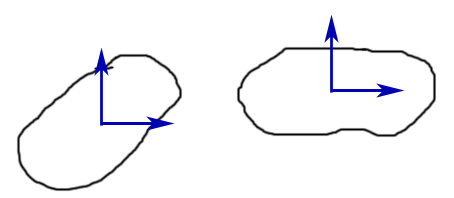
\includegraphics[width=0.30\textwidth]{softArt_G1.png}
	\caption{two bones}
	\label{2 Bones}
\end{figure}


Each of these bones contains several articulations points, also defined by rigids to have orientation information. \textsl{cf fig. 2}
\begin{figure}[htpb]
	\centering
		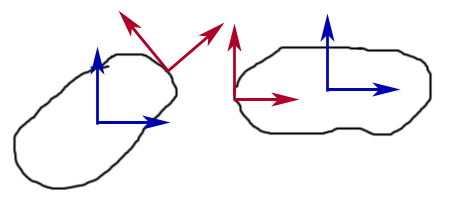
\includegraphics[width=0.30\textwidth]{softArt_G2.png}
	\caption{two bones (blue) with their articulation frames (red)}
\end{figure}

As seen previously, a joint between 2 bones is modeled by a 6-DOF spring. These springs are attached on the articulations points.    \textsl{cf fig. 3}
\begin{figure}[htpb]
	\centering
		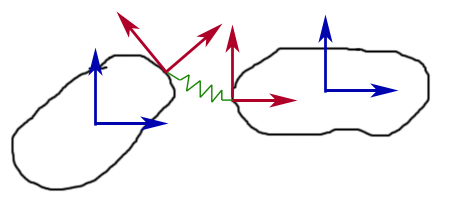
\includegraphics[width=0.30\textwidth]{softArt_G3.png}
	\caption{two bones linked by a joint-spring}
\end{figure}



\subsection{Sofa implementation}

To simulate these components in Sofa, we first need 2 mechanical objects : one for the bones (independent DOFs), and an other for the articulation points (mapped DOFs).
Each of them contains a list of rigid DOFs (respectively all the bones and all the articulations of the articulated body).
A mapping performs the link between the two lists, to know which articulations belong to which bones.


\subsubsection{Corresponding scene graph}
\begin{figure}[htpb]
	\centering
		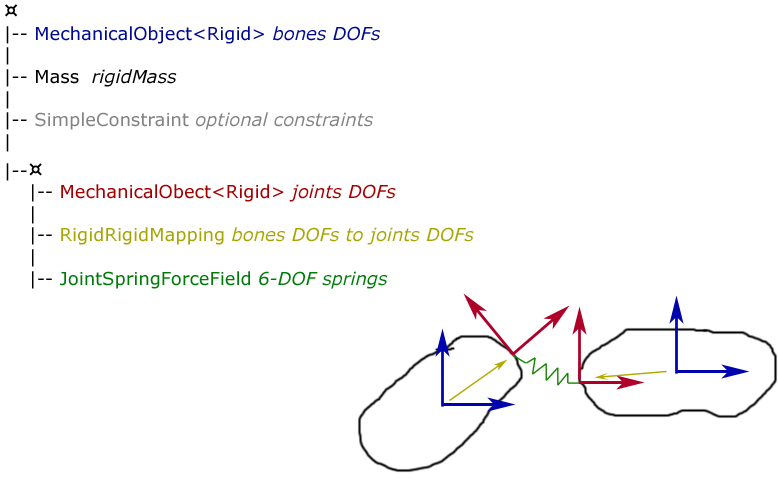
\includegraphics[width=0.90\textwidth]{scene_graph.png}
	\caption{a simple articulated body scene}
\end{figure}

\subsubsection {Example}

The example softArticulations.scn shows a basic pendulum :

\begin{verbatim}
<Node>
  <Object type="BruteForceDetection"/>
  <Object type="DefaultContactManager"/>
  <Object type="DefaultPipeline"/>
  <Object type="ProximityIntersection"/>

  <Node>
    <Object type="CGImplicitSolver"	/>
    <Object type="MechanicalObject" template="Rigid" name="bones DOFs"
            position="0 0 0  0 0 0 1 
                      1 0 0  0 0 0 1 
                      3 0 0  0 0 0 1 
                      5 0 0  0 0 0 1 
                      7 0 0  0 0 0 1" />
    <Object type="UniformMass" template="Rigid" name="bones mass"
            mass="1 1 [1 0 0,0 1 0,0 0 1]" />
    <Object type="FixedConstraint" template="Rigid" name="fixOrigin"
            indices="0" />
		
    <Node>
      <Object type="MechanicalObject" template="Rigid" name="articulation points"
              position="0 0 0  0.707914 0 0 0.707914 
                       -1 0 0  0.707914 0 0 0.707914 
                        1 0 0  0.707914 0 0 0.707914 
                       -1 0 0  0.707914 0 0 0.707914 
                        1 0 0  0.707914 0 0 0.707914 
                       -1 0 0  0.707914 0 0 0.707914 
                        1 0 0  0.707914 0 0 0.707914 
                       -1 0 0  0.707914 0 0 0.707914 
                        1 0 0  0.707914 0 0 0.707914" />
      <Object type="RigidRigidMapping"
              repartition="1 2 2 2 2" />
      <Object type="JointSpringForceField" template="Rigid" name="joint springs"
              spring="0 1   0 0 0 0 1 0   0 30000  0 200000   0  0 0 0  0 0 0 1 
                      2 3   0 0 0 0 1 0   0 30000  0 200000   0  0 0 0  0 0 0 1
                      4 5   0 0 0 0 1 0   0 30000  0 200000   0  0 0 0  0 0 0 1
                      6 7   0 0 0 0 1 0   0 30000  0 200000   0  0 0 0  0 0 0 1" />
    </Node>
    <Node>
      <Object type="MechanicalObject" template="Vec3d"
              position="-1 -0.5 -0.5  -1 0.5 -0.5 ..." />
      <Object type="MeshTopology"
              lines="0 1  1 2  ..."
              triangles="3 1 0  3 2 1  ..." />
      <Object type="TriangleModel"/>
      <Object type="LineModel"/>
      <Object type="RigidMapping"
              repartition="0 8 8 8 8" />
    </Node>
  </Node>
</Node>

\end{verbatim}

\begin{figure}[htpb]
	\centering
		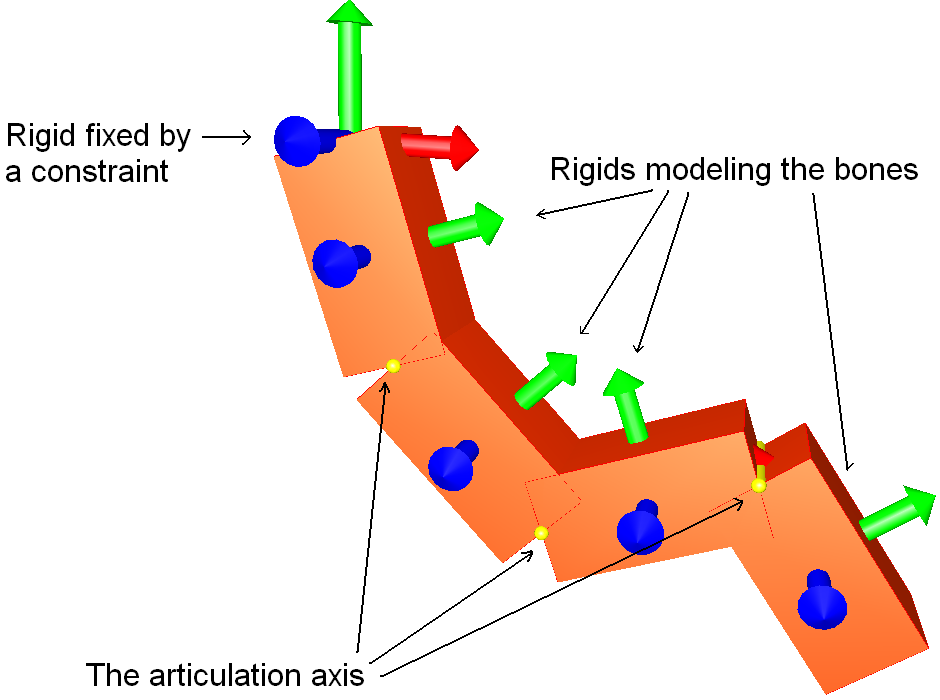
\includegraphics[width=0.70\textwidth]{softArt_snapshot.png}
	\caption{The pendulum is composed by 4 rigids linked one by one by articulations}
\end{figure}

In this example, we have under the first node the components to manage collisions, as usual.
Under the second node, we have :
\begin{itemize}
	\item the solver,
	\item the mechanical object modeling the independent rigid DOFs (5 rigids here),
	\item the rigid mass,
	\item a constraint, to fix the first rigid.
\end{itemize}

The third node (a child of the previous one) contains the components relative to the articulations :
\begin{itemize}
	\item the mechanical object modeling articulation points. Positions and orientations are relative to their parents.
	\item the mapping to link the two mechanical objects, as explained before. To know which articulations belong to which bones, a repartition vector is used. Several cases for this vector are possible :
		\begin{itemize}
			\item no value specified : every articulations belong to the first bone (classic rigid mapping).
			\item one value specified (ex: repartition="2") : each bone has the same number of articulations.
			\item number of bones values (like here, repartition="1 2 2 2 2") : the number of articulations is specified for each bone. For instance, here the first bone has 1 articulation, the next has 2 articulations, the next 2, Etc.
		\end{itemize}
	\item the JointSpringForceField containing the springs (4 springs here). Each spring is defined by a list of parameters. For instance for the first spring we have "0 1   0 0 0 0 1 0   0 30000  0 200000   0  0 0 0  0 0 0 1".
		\begin{itemize}
			\item "0 1" are the indices of the two articulations the spring is attached to
			\item "0 0 0 0 1 0" design the free axis for the movements. "0 0 0" mean that the 3 translation axis are constrained, and "0 1 0" mean that only the Y rotation axis is free.
			\item "0 30000 0 2000000" are the stiffnesses for each kind of movement: "0 30000" are respectively for free translation and for constrained translation", and "0 2000000" are respectively for free rotation and for constrained rotation.
			\item "0" is the damping factor
			\item "0 0 0" is to specify the initial translation
			\item "0 0 0 1" is to specify the initial rotation (quaternion)
		\end{itemize}
\end{itemize}

The last node contains the collision model. Nothing special here.


\subsection{Skinning}

The articulated body described previously models the skeleton of an object.
To have the external model (for the visual model or the collision model), which follows correctly the skeleton movements, it has to be mapped with the skeleton. 
\ 
A skinning mapping allows us to do this link. The external model is from this moment to deform itself smoothly, i.e. without breaking points around the articulations.

The influence of the bones on each point of the external model is given by skinning weights.
2 ways are possible to set the skinning weights to the mapping :
\begin{itemize}
	\item Either the user gives directly the weights list to the mapping. It is useful if good weights have been pre computed previsouly, like in Maya for instance.
	\item Else, the user defines a number of references \textsl{n} that will be used for mapped points. Then, each external model point will search its \textsl{n} nearest bones (mechanical DOFs), and then compute the skinning weights from the relation :
\[ W = \frac{1}{d^{2}}  \]
\small{ with \textsl{d} : the distance between the external point and the rigid DOF.}
\end{itemize}

\begin{figure*}[htpb]
		\centering
		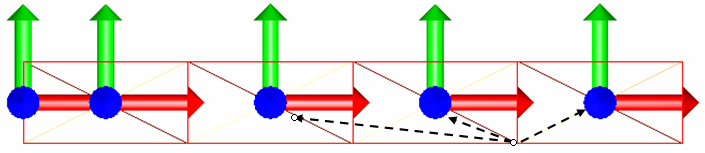
\includegraphics[width=0.50\textwidth]{skinning}
		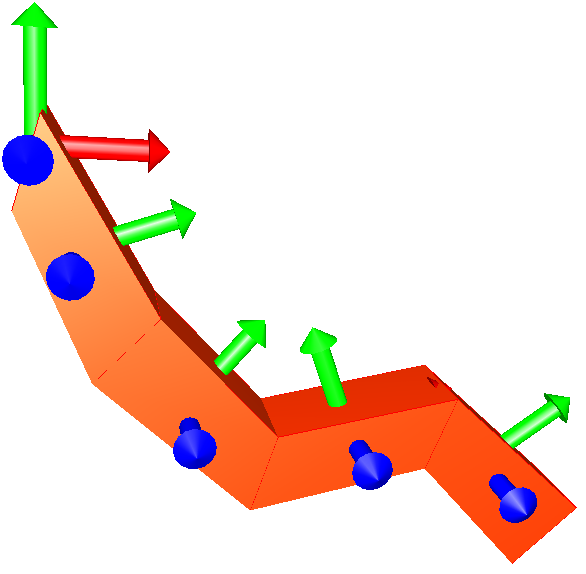
\includegraphics[width=0.30\textwidth]{skinnedPendulum}	
	\caption{In the example "softArticulationsSkinned.scn" the external points compute their skinning weights from the 3 nearest DOFs}
\end{figure*}



\end{document}          

